\chapter{System Description and Research}
\begin{comment}
Depending on the nature of the problem, this chapter should present the following briefly and in a way that the ideas for solutions, new concepts, process optimisation, results and conclusions can be understood and accepted by appropriately qualified readers:

consider here a chapter like sw dev with model based design 
reference: https://webthesis.biblio.polito.it/12441/1/tesi.pdf

>> detailed hw explain maybe also its hw arch
\begin{itemize}
	\item The theoretical basis used in your thesis
	\item Acknowledged methods of calculation and processes
	\item Methodological regulations and concepts (\eg VDI standard 2221 ``Methodological design'', TQM/TPM concept, ABC analysis, standards, \etc)
	\item Technological and physical foundation (material issues, manufacturing processes, physical laws, \etc)
	\item Economic methods and figures
	\item Legal basis
\end{itemize}
\end{comment}

\section{System Structure and Components}

The adaptive headlight software system is designed to dynamically adjust vehicle lighting, enhancing safety and visibility. At its core, the system leverages real-time telemetry inputs to assess vehicle dynamics, information about the driving environment  and driver inputs. These inputs are processed by the Light Control Unit (LCU), the decision-making hub equipped with advanced software.
\begin{figure}[h!]
    \centering
    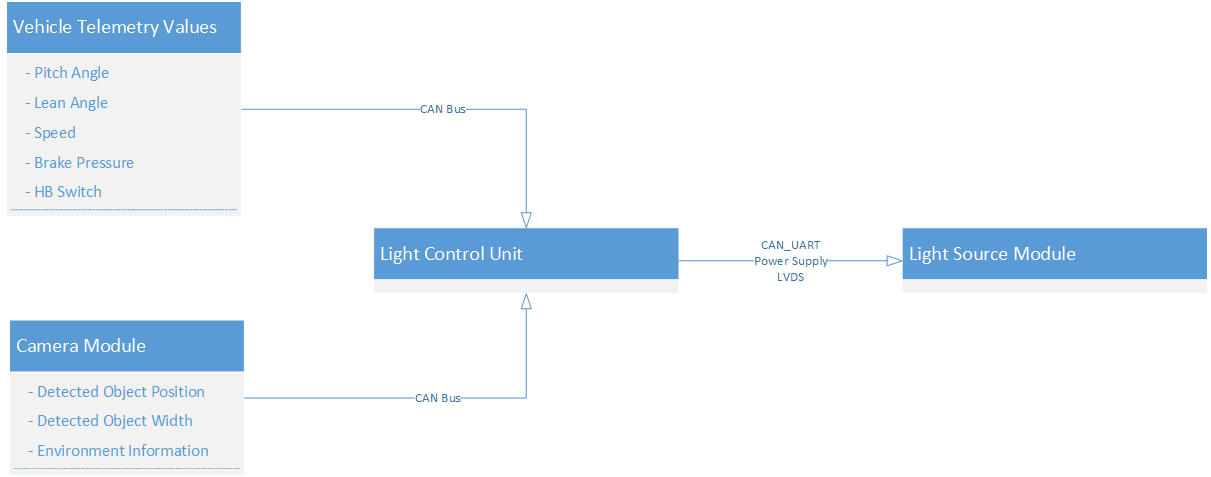
\includegraphics[width=0.75\linewidth]{Grafik/Overview_system_structure.png}
    \caption{The overview of the system structure}
    \label{fig:enter-label}
\end{figure}
The LCU orchestrates the operation of the Light Source Module (LSM), which utilizes HD matrix technology in the headlights. This technology allows for detailed adjustments in lighting patterns and intensity, tailoring illumination to suit varied driving environments and scenarios. Below is a simplified overview of the system structure, with further details provided in the following sections.
\subsection{Telemetry Values}
Telemetry inputs provide real-time data about the vehicle's movement and user inputs, enabling the system to adjust lighting conditions dynamically. Some of the main telemetry inputs used in the system include:

\begin{itemize}
    \item Lean Angle: Detects the side-to-side orientation of the vehicle.
    \item Pitch Angle: Detects the vehicle's front-to-back orientation.
    \item HB \& LB Signal: Tracks manual activation of high/low beams.
    \item Speed: Measures the vehicle's speed.
    \item Brake Pressure: Monitors brake activation.
    \item Ambient Light Sensor: Gauges external light levels.
\end{itemize}


These telemetry values are used in control logic to adjust each pixel, providing optimal illumination based on the current driving conditions.

\subsection{Camera Module}
To provide a glare-free high beam capability, vehicle detection is necessary to interpret traffic conditions. For this purpose, a camera module is mounted on the front of the motorcycle. This module includes the camera hardware, a software/firmware processing unit, and I/O interfaces that provide information via the CAN protocol. The key functionalities of the camera module for the adaptive headlight software are:

\begin{itemize}
    \item Object Detection: The system can detect up to 10 objects, categorizing them as either followed or approaching vehicles. To prevent glare, the pixels corresponding to these vehicles are completely shut off.
    \item Object Coordinates: Outputs the center coordinates and width of detected objects. The height is not considered as it does not impact road illumination.
    \item Environmental Information: Detects whether the vehicle is driven in specific conditions such as village areas, foggy conditions, or speed-limited zones. This information helps in providing Automated High Beam (AHB) functionality, particularly when the pixel HD matrix headlight is not available for mid and lower-end motorcycles.
\end{itemize}
In the following sections, the control software, logic, image creation, and system output, as well as detailing how these inputs are processed and utilized to optimize headlight performance will be discussed.


\section{Light Control Unit}
The Light Control Unit (LCU) serves as the core of the pixel headlight system, acting as both the system's brain and its central algorithmic processor. It processes real-time telemetry inputs, analyzes vehicle dynamics, and assesses environmental conditions to accurately modulate the headlight's output. The inputs to the LCU are CAN messages as previously mentioned. The output of the LCU is a grey-scale 2D array generated at each time step, with each element representing a pixel of the light source unit.

A software architecture and  UML diagram have been developed to optimally orchestrate the light source unit. The control software, flashed onto the LCU, incorporates the Ethernet Protocol (ETH) and User Datagram Protocol (UDP), ensuring reliable transmission of lighting commands to the light source unit.
The LCU's hardware includes dedicated PWM outputs for precise light intensity control, supporting Low Beam (LB) and High Beam (HB) headlights, each capable of handling up to 3 Amperes. This versatility allows management of Front Position Lamp (FPL) and Daytime Running Lights (DRL), with outputs rated at 200 milliamperes and 3 Amperes, respectively.

Additionally, the LCU features dual CAN interfaces for robust vehicle-wide communication and an LVDS interface for high-speed data or video signal transmission. These communication technologies are critical for exchanging control signals, enabling real-time lighting adjustments to meet the dynamic needs of the vehicle and its environment. This network of communication channels facilitates data transfer and integration between the LCU and the Light Source Module (LSM), enhancing interaction between the vehicle, driver, and environment while ensuring immediate lighting responses.

\section{Light Source Unit}
LSU in this project, also known as the HD Matrix LED Pixel
High Beam Headlight or simply 'pixel headlight,' is one of the main parts of the
vehicle's headlight system.

The input to the Light Source Unit (LSU) is a grey-scale image array integrated with the communication protocol (UDP+ETH), representing light illumination as processed by the software. The LCU uses telemetry data to direct the LSU to modify its lighting pattern, intensity, and direction, ensuring optimal adaptation to prevailing driving conditions. These continuous adjustments significantly enhance visibility and safety. Such continuous adjustments improve visibility and safety.

Key features of the LSU include:
\begin{itemize}
    \item Matrix Pixel LED Technology: Featuring a 64x256 matrix, the LSU houses 16,384 individually controllable LED pixels. This advanced technology allows for dynamic beam shaping, enhancing adaptability and safety in various driving environments. \cite{7_Internal_Doc_HELLA}
    \item SSL HD System: Utilizing Solid State Lighting (SSL) with High Definition (HD) capabilities, the LSU achieves detailed clarity and precision in its illumination pattern. This high-resolution technology ensures the light output is highly adaptable to different scenarios. \cite{7_Internal_Doc_HELLA}
    \item Beam Horizontal Angle: The SSL HD system provides various beam spreads, such as the "26°" model, offering a focused beam narrower than the average low-beam module. While this provides concentrated illumination, it also presents challenges in covering all areas typically illuminated by the low beam. \cite{7_Internal_Doc_HELLA}
\end{itemize}


Overall, the integration of the LSU with the LCU, supported by advanced lighting technology and real-time data processing, results in a headlight system that delivers optimal illumination tailored to real-time driving scenarios.







\section{Development for Embedded Applications}
% how to develop model-based systems for embedded applications
% 		○ Embedded environment,  Software engineer will often   directly to the microprocessor  without using a OS




\subsection{Characteristics of Embedded System}

\subsection{Real-Time Implementation}

\subsection{Code Generation and Deployment}








\newpage

\section{Vehicle Detection Algorithm}

\subsection{Overview}
\textit{". At present, the YOLO series is one of the most excellent algorithms in single-stage detection; it has the characteristics of a smaller parameter count, high detection accuracy, and high speed. Therefore, it is widely used in vehicle inspection"} \cite{Yolov5_Improvement}

\begin{figure}[h!]
    \centering
    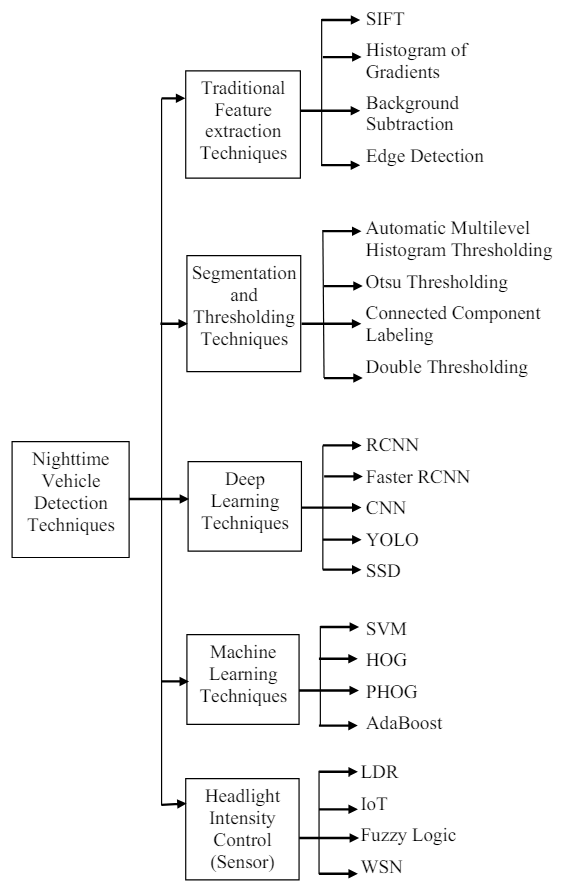
\includegraphics[width=0.75\linewidth]{Vehicle_detect_classification_nighttime.png}
    \caption{Classification of the techniques for nighttime vehicle identification and headlight intensity control. \cite{night_vehicle_detec}}
    \label{fig:enter-label}
\end{figure}


\subsection{Our Strategy - YOLOv5}

%https://www.mdpi.com/1424-8220/24/4/1182 \cite{Yolov5_Improvement}


\newpage
\section{Transformation Algorithm for Alignment}

\subsection{Rigid Body Transformation}
